\documentclass[12pt,letterpaper]{exam}
\usepackage[lmargin=1in,rmargin=1in,tmargin=1in,bmargin=1in]{geometry}
\usepackage{../style/exams}

% -------------------
% Course & Exam Information
% -------------------
\newcommand{\course}{MAT 101: Exam 1}
\newcommand{\term}{Spring -- 2022}
\newcommand{\examdate}{03/10/2022}
\newcommand{\timelimit}{85 Minutes}

\setbool{hideans}{false} % Student: True; Instructor: False

% -------------------
% Content
% -------------------
\begin{document}

\examtitle
\instructions{Write your name on the appropriate line on the exam cover sheet. This exam contains \numpages\ pages (including this cover page) and \numquestions\ questions. Check that you have every page of the exam. Answer the questions in the spaces provided on the question sheets. Be sure to answer every part of each question and show all your work.} 
\scores
%\bottomline
\newpage

% ---------
% Questions
% ---------
\begin{questions}

% Question 1
\question[10] Mark each  of the following statements as True ($T$) or False ($F$). \pspace
\begin{enumerate}[(a)]
\item \underline{\itshape\hspace{0.6cm}T\hspace{0.6cm}}: $4^{100} + 4^{100} + 4^{100} + 4^{100}= 4^{101}$. \vfill
\item \underline{\itshape\hspace{0.65cm}F\hspace{0.65cm}}: The number 1 is a multiple of 12. \vfill
\item \underline{\itshape\hspace{0.6cm}T\hspace{0.6cm}}: The number 4 has three divisors. \vfill
\item \underline{\itshape\hspace{0.65cm}F\hspace{0.65cm}}: The number 1 is prime. \vfill
\item \underline{\itshape\hspace{0.6cm}T\hspace{0.6cm}}: Every integer greater than 1 is a product of prime numbers. \vfill
\item \underline{\itshape\hspace{0.65cm}F\hspace{0.65cm}}: For all real numbers $x$, we know $x^0= 1$. \vfill
\item \underline{\itshape\hspace{0.6cm}T\hspace{0.6cm}}: There is no rational number equal to $\pi$. \vfill
\item \underline{\itshape\hspace{0.65cm}F\hspace{0.65cm}}: The number $31.2 \cdot 10^5$ is in scientific notation. \vfill
\item \underline{\itshape\hspace{0.6cm}T\hspace{0.6cm}}: Two lines with positive slopes can never be perpendicular. \vfill
\item \underline{\itshape\hspace{0.65cm}F\hspace{0.65cm}}: The line $y= x + 6$ is parallel to the line $y= 7 - x$. \vfill
\end{enumerate}



\newpage



% Question 2
\question[8] Find the prime factorization for each of the following integers: \pspace
        \begin{enumerate}[(a)]
        \item $126=  2 \cdot 3^2 \cdot 7$ \pspace
        	\[
	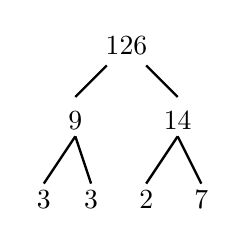
\begin{tikzpicture}
	\node at (-0.15,0.15) {$126$};
	\draw[line width=0.03cm] (-0.4,-0.1) -- (-0.8,-0.5);
	\node at (-0.8,-0.8) {$9$};
	\draw[line width=0.03cm]  (0.1,-0.1) -- (0.5,-0.5);
	\node at (0.5,-0.8) {$14$};
		
	\draw[line width=0.03cm] (-0.8,-1) -- (-1.2,-1.6);
	\node at (-1.2,-1.8) {$3$};
	\draw[line width=0.03cm] (-0.8,-1) -- (-0.6,-1.6);
	\node at (-0.6,-1.8) {$3$};
	
	\draw[line width=0.03cm] (0.5,-1) -- (0.1,-1.6);
	\node at (0.1,-1.8) {$2$};
	\draw[line width=0.03cm] (0.5,-1) -- (0.8,-1.6);
	\node at (0.8,-1.8) {$7$};
	\end{tikzpicture}
	\] \pvspace{0.9cm}
	
        \item $37= 37^1$ \vfill
        \item $120= 2^3 \cdot 3 \cdot 5$ 
        
        	\[
	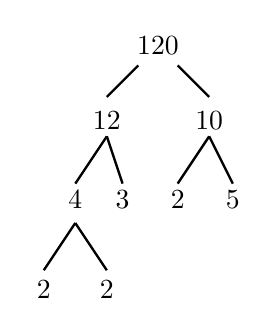
\begin{tikzpicture}
	\node at (-0.15,0.15) {$120$};
	\draw[line width=0.03cm] (-0.4,-0.1) -- (-0.8,-0.5);
	\node at (-0.8,-0.8) {$12$};
	\draw[line width=0.03cm]  (0.1,-0.1) -- (0.5,-0.5);
	\node at (0.5,-0.8) {$10$};
		
	\draw[line width=0.03cm] (-0.8,-1) -- (-1.2,-1.6);
	\node at (-1.2,-1.8) {$4$};
		\draw[line width=0.03cm] (-1.2,-2.1) -- (-1.6, -2.7);
		\draw[line width=0.03cm] (-1.2,-2.1) -- (-0.8,-2.7);
		\node at (-1.6,-2.95) {$2$};
		\node at (-0.8,-2.95) {$2$};
	\draw[line width=0.03cm] (-0.8,-1) -- (-0.6,-1.6);
	\node at (-0.6,-1.8) {$3$};
	
	\draw[line width=0.03cm] (0.5,-1) -- (0.1,-1.6);
	\node at (0.1,-1.8) {$2$};
	\draw[line width=0.03cm] (0.5,-1) -- (0.8,-1.6);
	\node at (0.8,-1.8) {$5$};
	\end{tikzpicture}
	\] \pvspace{0.1cm}
	
        \item $141=  3 \cdot 47$ 
	\[
	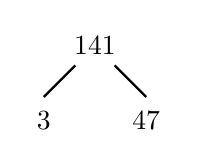
\begin{tikzpicture}
	\node at (-0.15,0.15) {$141$};
	\draw[line width=0.03cm] (-0.4,-0.1) -- (-0.8,-0.5);
	\node at (-0.8,-0.8) {$3$};
	\draw[line width=0.03cm]  (0.1,-0.1) -- (0.5,-0.5);
	\node at (0.5,-0.8) {$47$};
	\end{tikzpicture}
	\] \pvspace{2.9cm}
        \end{enumerate}



\newpage



% Question 3
\question[8] Compute the following: \pspace
        \begin{enumerate}[(a)]
        \item $\gcd(28, 70)= \gcd(2^2 \cdot 7, 2 \cdot 5 \cdot 7)= 2 \cdot 7= 14$ \vfill
        \item $\lcm(28, 70)= \lcm(2^2 \cdot 7, 2 \cdot 5 \cdot 7)= 2^2 \cdot 5 \cdot 7= 140$ \vfill
        \item $\gcd(2^{500} \cdot 3^{98} \cdot 11^{82} \cdot 53^{17},\, 2^{200} \cdot 3^{50} \cdot 7^{60} \cdot 13^{300})= 2^{200} \cdot 3^{50}$ \vfill
        \item $\lcm(2^{500} \cdot 3^{98} \cdot 11^{82} \cdot 53^{17},\, 2^{200} \cdot 3^{50} \cdot 7^{60} \cdot 13^{300})= 2^{500} \cdot 3^{98} \cdot 7^{60} \cdot 11^{82} \cdot 13^{300} \cdot 53^{17}$ \vfill
        \end{enumerate}



\newpage



% Question 4
\question[8] Showing all your work and simplifying as much as possible, compute the following: \pspace
	\begin{enumerate}[(a)]
	\item $\dfrac{5}{12} - \dfrac{3}{4}= \dfrac{5}{12} - \dfrac{9}{12}= -\dfrac{4}{12}= -\dfrac{1}{3}$ \vfill
	\item $\dfrac{11}{6} + \dfrac{4}{15}= \dfrac{55}{30} + \dfrac{8}{30}= \dfrac{63}{30}= \dfrac{21}{10}$ \vfill
	\item $\dfrac{12}{55} \cdot \dfrac{5}{6}= \dfrac{\cancel{12}^2}{\cancel{55}^{11}} \cdot \dfrac{\cancel{5}^1}{\cancel{6}^1}= \dfrac{2}{11}$ \vfill
	\item $\dfrac{\;\;\dfrac{20}{21}\;\;}{\dfrac{8}{7}}= \dfrac{20}{21} \cdot \dfrac{7}{8}= \dfrac{\cancel{20}^5}{\cancel{21}^3} \cdot \dfrac{\cancel{7}^1}{\cancel{8}^2}= \dfrac{5}{6}$ \vfill
	\end{enumerate}



\newpage



% Question 5
\question[8] Showing all your work and being sure to use no negative powers, simplify the following as much as possible: \pspace
	\begin{enumerate}[(a)]
	\item $\left( \dfrac{x^3 (x^2y^5)^0}{y^7} \right)^{-2}= \left( \dfrac{y^7}{x^3 (x^2y^5)^0} \right)^2= \dfrac{y^{14}}{x^6 (x^2y^5)^0}= \dfrac{y^{14}}{x^6}$ \vfill
	\item $\dfrac{(x^2 y^3)^3}{x^{10} y^{-5}}= \dfrac{x^6 y^9}{x^{10} y^{-5}}= \dfrac{x^6 y^9 y^5}{x^{10}}= \dfrac{\cancel{x^6} y^{14}}{x^{\cancel{10}^4}}= \dfrac{y^{14}}{x^4}$ \vfill
	\item $(\sqrt{x^5}\, y^{-3})^4= (x^{5/2} y^{-3})^4= x^{20/2}\, y^{-12}= \dfrac{x^{10}}{y^{12}}$ \vfill
	\item $\left( \dfrac{x^6}{y^5} \right)^{-1/3}= \left( \dfrac{y^5}{x^6} \right)^{1/3}= \dfrac{y^{5/3}}{x^{6/3}}= \dfrac{\sqrt[3]{y^5}}{x^2}$ \vfill
	\end{enumerate}



\newpage



% Question 6
\question[8] Simplify the following radical expressions: \pspace
	\begin{enumerate}[(a)]
	\item $\sqrt{36}= \sqrt{6^2}= 6$ \vfill
	\item $\sqrt[3]{64}= \sqrt[3]{4^3}= 4$ \vfill
	\item $\sqrt{2^5 \cdot 3^2 \cdot 5}= 2 \cdot 2 \cdot 3 \sqrt{2 \cdot 5}= 12 \sqrt{10}$ \vfill
	\item $\sqrt[4]{2^3 \cdot 3^9 \cdot 5^4}= 3 \cdot 3 \cdot 5 \sqrt[4]{2^3 \cdot 3}= 45 \sqrt[4]{24}$ \vfill
	\end{enumerate}



\newpage



% Question 7
\question[6] Showing all your work and simplifying as much as possible, rationalize the following: \pspace
	\begin{enumerate}[(a)]
	\item $\dfrac{4}{\sqrt{6}}= \dfrac{4}{\sqrt{6}} \cdot \dfrac{\sqrt{6}}{\sqrt{6}}= \dfrac{4 \sqrt{6}}{6}= \dfrac{2 \sqrt{6}}{3}$ \vfill
	\item $\dfrac{1}{\sqrt[3]{7}}= \dfrac{1}{7^{1/3}}= \dfrac{1}{7^{1/3}} \cdot \dfrac{7^{2/3}}{7^{2/3}}= \dfrac{\sqrt[3]{7^2}}{7^{1/3 + 2/3}}= \dfrac{\sqrt[3]{49}}{7}$ \vfill
	\item $\dfrac{1}{3 - \sqrt{5}}= \dfrac{1}{3 - \sqrt{5}} \cdot \dfrac{3 + \sqrt{5}}{3 + \sqrt{5}}= \dfrac{3 + \sqrt{5}}{9 + 3 \sqrt{5} - 3 \sqrt{5} - 5}= \dfrac{3 + \sqrt{5}}{9 - 5}= \dfrac{3 + \sqrt{5}}{4}$ \vfill
	\end{enumerate}



\newpage



% Question 8
\question[8] Showing all your work, convert 5~km/s$^2$ to miles per square minute. Note that 1~km $=$ 1000~m, 1~ft $=$ 0.3048~m, and 60~s $=$ 1~min.

	\begin{table}[!ht]
	\centering
	\begin{tabular}{c|c|c|c|c}
	$5$~km & $1000$~m & $1$~ft & $60$~s & $60$~s \\ \hline
	$1$~s$^2$ & $1$~km & $0.3048$~m & $1$~min & $1$~min$^2$
	\end{tabular}
	$= 59055120.0$~mi/min$^2$
	\end{table}



\newpage



% Question 9
\question[4] Complete the following:
	\begin{enumerate}[(a)]
	\item Convert the following number in scientific notation to an ordinary \par decimal number: $-4.73 \cdot 10^{-6}$ \pspace
		\[
		-4.73 \cdot 10^{-6}= -0.00000473
		\] \pvspace{0.85cm}
	\item Convert the following ordinary decimal number to scientific notation: $0.054$ \pspace
		\[
		0.054= 5.4 \cdot 10^{-2}
		\] \pvspace{0.85cm}
	\end{enumerate} \vfill

% Question 10
\question[8] Showing all your work, compute the following: \pspace
        \begin{enumerate}[(a)]
        \item 97 decreased by 60\% \pspace
		\[
		97 (1 - 0.60)= 97(0.40)= 38.8
		\] \pvspace{0.85cm}
	
        \item 573 increased by 142\% \pspace
		\[
		573 (1 + 1.42)= 573(2.42)= 1386.66
		\] \pvspace{0.85cm}
	
        \item 71\% of 140 \pspace
		\[
		140 (0.71)= 99.4 
		\] \pvspace{0.9cm}
        \end{enumerate}



\newpage



% Question 11
\question[8] Compute the following, being sure to show all your work and to write your answer in the form $a + bi$: \pspace
	\begin{enumerate}[(a)]
	\item $(3i)^3= 3^3 \cdot i^3= 27(-i)= -27i= 0 - 27i$ \vfill
	\item $(6 + 4i) - (4 - 4i)= (6 - 4) + \big(4i - (-4i) \big)= 2 + 8i$ \vfill
	\item $(1 + i)(3 - 2i)= 3 - 2i + 3i - 2i^2= 3 + i - 2(-1)= 3 + 2 + i= 5 + i$ \vfill
	\item $\dfrac{6 + i}{1 - i}= \dfrac{6 + i}{1 - i} \cdot \dfrac{1 + i}{1 + i}= \dfrac{6 + 6i + i + i^2}{1 + i - i - i^2}= \dfrac{6 + 7i - 1}{1 - (-1)}= \dfrac{5 + 7i}{2}$ \vfill
	\end{enumerate}



\newpage



% Question 12
\question[8] Suppose a student has a 90\% participation average, 75\% quiz average, 84\% homework average, 86\% on the midterm, and 66\% on the final exam, given that their course grade is computed using the weights below, find their course average:
	\begin{table}[!ht]
	\centering
	\begin{tabular}{rr}
	Participation: & 5\% \\
	Quizzes: & 15\% \\
	Homework: & 45\% \\
	Midterm: & 15\% \\
	Final: & 20\%
	\end{tabular}
	\end{table} \pspace

	\[
	\begin{aligned}
	\text{Course Average}&= \sum \text{Grade Component} \cdot \text{Average (Decimal)} \\[0.3cm]
	&= 5 (0.90) + 15(0.75) + 45(0.84) + 15(0.86) + 20(0.66) \\[0.3cm]
	&= 4.5 + 11.25 + 37.8 + 12.9 + 13.2 \\[0.3cm]
	&= 79.65
	\end{aligned}
	\]



\newpage



% Question 13
\question[8] Answer the following:
	\[
	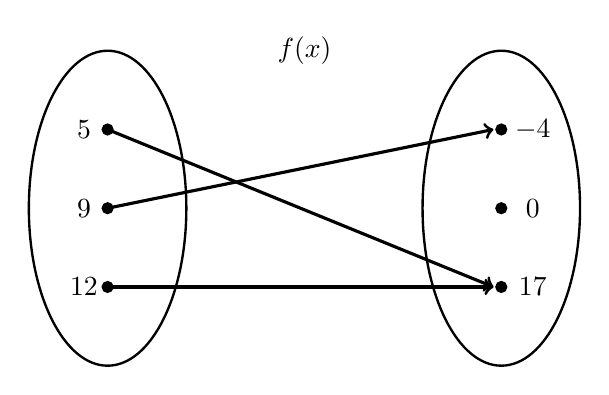
\begin{tikzpicture}
	\node at (2.5,2) {$f(x)$};
	% Ellipses
	\draw[line width=0.03cm] (0,0) circle (1 and 2);
	\draw[line width=0.03cm] (5,0) circle (1 and 2);
	
	% Nodes
	\draw[fill=black] (0,1) circle (0.07);
	\draw[fill=black] (0,0) circle (0.07);
	\draw[fill=black] (0,-1) circle (0.07);
	
	\draw[fill=black] (5,1) circle (0.07);
	\draw[fill=black] (5,0) circle (0.07);
	\draw[fill=black] (5,-1) circle (0.07);
	
	% Arrow
	\draw[line width=0.04cm,->] (0,1) -- (4.9,-1);
	\draw[line width=0.04cm,->] (0,0) -- (4.9,1);
	\draw[line width=0.04cm,->] (0,-1) -- (4.9,-1);
	
	% Labels
	\node at (-0.3,1) {$5$};
	\node at (-0.3,0) {$9$};
	\node at (-0.3,-1) {$12$};
	
	\node at (5.4,1) {$-4$};
	\node at (5.4,0) {$0$};
	\node at (5.4,-1) {$17$};
	\end{tikzpicture}
	\] \pspace

\begin{enumerate}[(a)]
\item Explain why the relation $f(x)$ above is a function. \pvspace{1.9cm}

{\itshape For each input, there is only one possible output, e.g. $f(5)= 17$, $f(9)= -4$, and $f(12)= 17$.} \pvspace{1.9cm}

\item Find the domain, codomain, and range of the function $f(x)$. \pvspace{0.8cm}
	\[
	\begin{aligned}
	\text{Domain}&= \{ 5, 9, 12 \} \\[0.3cm]
	\text{Codomain}&= \{ -4, 0, 17 \} \\[0.3cm]
	\text{Range}&= \{ -4, 17 \}
	\end{aligned}
	\] \pvspace{0.8cm}

\item Is the relation $g(x)= 17x - x^3$ a function? Explain. \pvspace{0.9cm}

{\itshape Yes, $g(x)$ is a function. This is because for each input, there is only one possible output---namely, the one obtained by evaluating $g(x)$ at $x$ and following order of operations.}
\end{enumerate}



\newpage



% Question 14
\question[8] Consider the relation $f(x)$ plotted below.
	\[
	\fbox{
	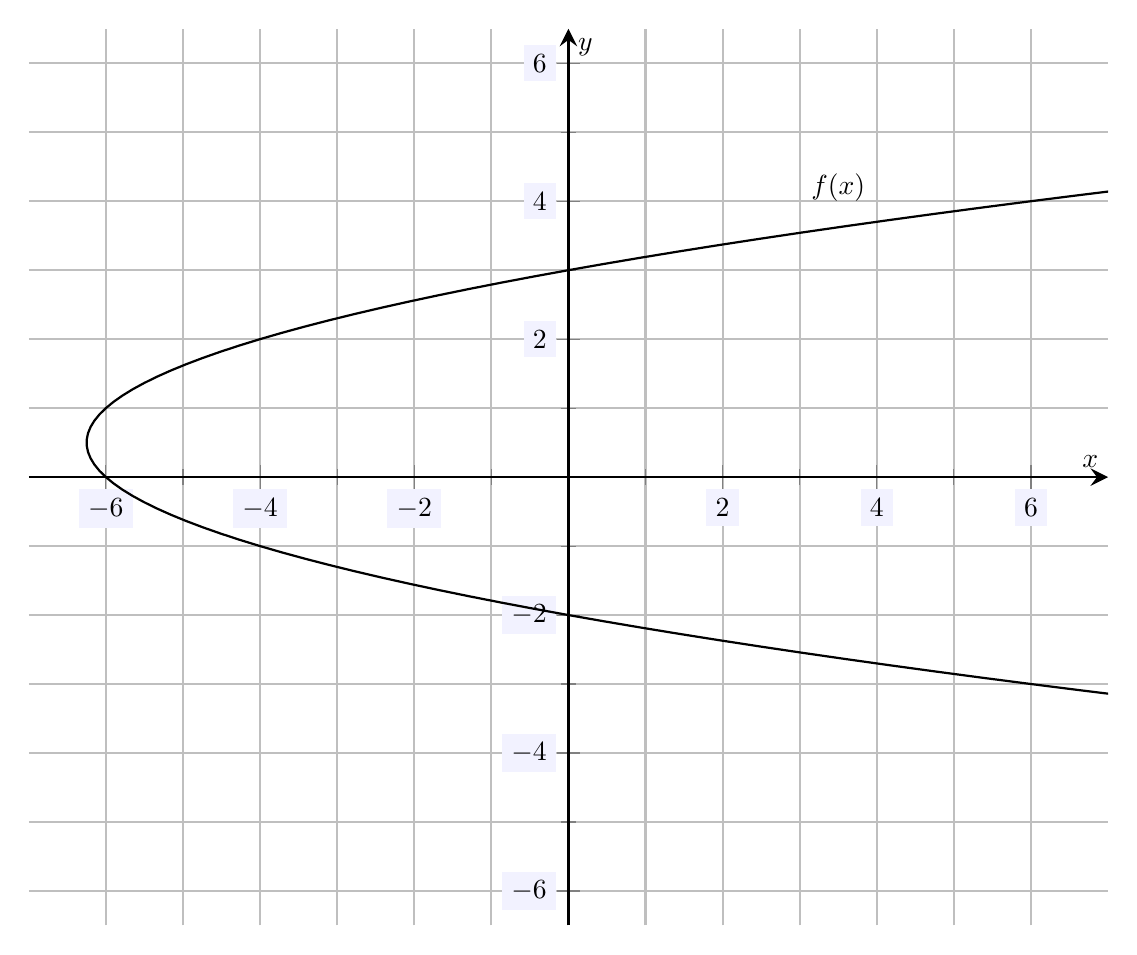
\begin{tikzpicture}[scale=2,every node/.style={scale=0.5}]
	\begin{axis}[
	grid=both,
	axis lines=middle,
	ticklabel style={fill=blue!5!white},
	xmin= -7, xmax=7,
	ymin= -6.5, ymax=6.5,
	xtick={-6,-4,-2,0,2,4,6},
	ytick={-6,-4,-2,0,2,4,6},
	minor tick = {-5,-3,...,5},
	xlabel=\(x\),ylabel=\(y\),
	]
	\node at (3.5,4.2) {$f(x)$};
	\addplot [domain= -4:5,samples=100] ({x^2 - x - 6},{x}); 
	\end{axis}
	\end{tikzpicture}
	}
	\] \pspace

\begin{enumerate}[(a)]
\item Is the relation $f(x)$ plotted above a function? Explain. \pvspace{0.3cm}

{\itshape No, $f(x)$ fails the vertical line test. For example, the input $x= 0$ has two possible outputs: $-2$ and $3$.} \pvspace{0.3cm}

\item Does the relation above have an inverse function? Explain. \pvspace{0.2cm}

{\itshape Yes, the relation $f(x)$ has an inverse function because it passes the horizontal line test, i.e. every horizontal line intersects the curve at most once.} \pvspace{0.2cm}

\item Find the $y$-intercepts of the relation plotted above. \pvspace{0.5cm}

{\itshape The $y$-intercepts are $y= -2, 3$, or more precisely the points $(0, -2)$ and $(0, 3)$.} \pvspace{0.5cm}

\item Find the $x$-intercepts of the relation plotted above. \pvspace{0.5cm}

{\itshape The only $x$-intercept is $x= -6$, or more precisely the point $(-6, 0)$.}
\end{enumerate}



\newpage



% Question 15
\question[6] Consider the functions given in the table below.
        \begin{table}[!ht]
        \centering
        \begin{tabular}{| c || r | r | r | r | r |} \hline
	$x$ & $-2$ & $-1$ & $0$ & $1$ & $2$ \\ \hline
	$f(x)$ & $5$ & $-2$ & $-5$ & $-3$ & $2$ \\ \hline
	$g(x)$ & $6$ & $2$ & $10$ & $7$ & $-5$ \\ \hline
        \end{tabular}
        \end{table}

Compute the following: \pspace
        \begin{enumerate}[(a)]
        \item $g(2)= -5$ \vfill
        \item $(f - g)(0)= f(0) - g(0)= -5 - 10= -15$ \vfill
        \item $(fg)(1)= f(1) g(1)= -3 \cdot 7= -21$ \vfill
        \item $\left( \dfrac{g}{f} \right)(0)= \dfrac{g(0)}{f(0)}= \dfrac{10}{-5}= -2$ \vfill
        \item $(f \circ g)(-1)= f(g(-1))= f(2)= 2$ \vfill
        \item $(g \circ f)(-1)= g(f(-1))= g(-2)= 6$ \vfill
        \end{enumerate}



\newpage



% Question 16
\question[8] Consider the function $\ell(x)= 6 - 2x$. \pspace
	\begin{enumerate}[(a)]
	\item Is $\ell(x)$ linear? Explain. \pvspace{1.4cm}
	
	{\itshape Yes, $\ell(x)$ is linear because it has the form $y= mx + b$ with $y= \ell(x)$, $x= x$, $m= -2$, and $b= 6$.} \pvspace{1.4cm}
	
	\item Find the slope of $\ell(x)$. \pvspace{1.3cm}
	
		\[
		m= -2
		\] \pvspace{1.3cm}
	
	\item Find the $y$-intercept of $\ell(x)$. \pvspace{1.3cm}
	
		\[
		y= 6 \text{ (or more precisely, $(0, 6) )$}
		\] \pvspace{1.3cm}
	
	\item Is the point $(-1, 4)$ on the graph of $\ell(x)$? Explain. \pvspace{1.3cm}
	
		\[
		\ell(-1)= 6 - 2(-1)= 6 - (-2)= 6 + 2= 8
		\] \pspace
	{\itshape Because $\ell(-1)= 8 \neq 4$, the point $(-1, 4)$ is not on the graph of $\ell(x)$.}
	\end{enumerate}



\newpage



% Question 17
\question[6] Find the equation of the line perpendicular to $y= 6 - 2x$ at its $x$-intercept. \pspace

{\itshape Because the line $y= 6 - 2x$ is not horizontal, we know that the line in question is not vertical. Therefore, our line must have the form $y= mx + b$. The line $y= 6 - 2x$ has slope $-2= -\frac{2}{1}$. Because our line is perpendicular to this line, it must have slope $m= -\left(-\frac{1}{2}\right)= \frac{1}{2}$. Then we know that $y= \frac{1}{2}\,x + b$. Our line contains the $x$-intercept of the line $y= 6 - 2x$. The $x$-intercept occurs when $y= 0$ so that we then have\dots
	\[
	\begin{aligned}
	0&= 6 - 2x \\[0.3cm]
	2x&= 6 \\[0.3cm]
	x&= 3
	\end{aligned}
	\]
Therefore, the $x$-intercept of $y= 6 - 2x$ is the point $(3, 0)$. But then we know\dots
	\[
	\begin{aligned}
	y&= \dfrac{1}{2}\,x + b \\[0.3cm]
	0&= \dfrac{1}{2} \cdot 3 + b \\[0.3cm]
	0&= \dfrac{3}{2} + b \\[0.3cm]
	b&= -\dfrac{3}{2}
	\end{aligned}
	\]
Therefore, the equation of the line is\dots
	\[
	\boxed{y= \dfrac{1}{2}\,x - \dfrac{3}{2}}
	\]
}



\newpage



% Question 18 
\question[6] Solve the following equation and then verify your solution:
	\[
	3x -14= 8 - \frac{2}{3}\,x
	\] \pspace
	
	\[
	\begin{aligned}
	3x -14&= 8 - \frac{2}{3}\,x \\[0.3cm]
	3(3x - 14)&= 3(8 - \frac{2}{3}\,x) \\[0.3cm]
	9x - 42&= 24 - 2x \\[0.3cm] 
	11x&= 66 \\[0.3cm]
	x&= 6
	\end{aligned}
	\] \pvspace{2cm}
	
	\[
	\begin{aligned}
	3x -14&= 8 - \frac{2}{3}\,x \\[0.3cm]
	3(6) - 14&\stackrel{?}{=} 8 - \frac{2}{3} \cdot 6 \\[0.3cm]
	18 - 14&\stackrel{?}{=} 8 - 4 \\[0.3cm]
	4&= 4 \\
	&\;\text{\cmark}
	\end{aligned}
	\]


\newpage



% Question 19
\question[8] You are driving home from university at 55~mph. Your home is 650~miles from your university. Assuming you left the university 2~hours ago and that you drive at a constant speed, find your distance from your home, $D(t)$, as function of time $t$, in hours. \pspace

{\itshape Let $t$ denote the amount of time (in hours) from the `current' hour and $D(t)$ be the distance (in miles) from home. Because you are driving at a constant rate of speed, we know that $D(t)$ is a linear function. Therefore, we must have $D(t)= mt + b$ for some $m$ and $b$. The rate of change is the slope, $m$. Because you are driving at 55~mph and because the distance between you and your home is decreasing, we must have $m= -55$. Therefore, we know $D(t)= -55t + b$. We also know 2~hours ago that you were 650~miles from home, i.e. that the point $(-2, 650)$ is on the graph of $D(t)$. But then\dots
	\[
	\begin{aligned}
	D(t)&= -55t + b \\[0.3cm]
	650&= -55(-2) + b \\[0.3cm]
	650&= 110 + b \\[0.3cm]
	b&= 540
	\end{aligned}
	\]
Therefore, we have\dots
	\[
	\boxed{D(t)= 540 - 55t}
	\] \vfill

Note: We could also use the fact that because you have driven two hours, you have traveled $55 \cdot 2= 110$~miles. So currently, i.e. at time $t= 0$, you are $650 - 110= 540$~miles from your home. But then $b= 540$. \pspace

Note: One could define $D(t)$ using the initial time, $t= 0$, to be the time at the start of the drive. Then because one's home is 650~miles from the school, we have $D(0)= 650$, which is the $y$-intercept $b$. We still have the rate of change being $m= -55$. But then $D(t)= 650 - 55t$. 
}



\newpage



% Question 20
\question[8] You rent an apartment in NYC, which you paid a \$50 application fee to apply for. The rent is \$2500/month. Therefore, the amount you have paid, $R(t)$, to rent the apartment $t$ months after moving in is given by $R(t)= 2500t + 50$.
	\begin{enumerate}[(a)]
	\item Without knowing $R(t)$, how do you know that $R(t)$ is linear? \pvspace{2.6cm}
	
	{\itshape The rate of change of the amount of money you have paid is constant, i.e. the monthly rent is fixed at a rate of \$2500/month. Therefore, $R(t)$ is linear.} \pvspace{2.6cm}

	\item What is the slope of $R(t)$ and what does it represent in the problem context? \pvspace{2.6cm}
	
	{\itshape Because $R(t)$ is linear, we know that the slope is $m= 2500$. In the context of the problem, this corresponds to the monthly rent payment of \$2,500.} \pvspace{2.6cm}
	
	\item What is the $y$-intercept of $R(t)$ and what does it represent in the problem context? \pvspace{2.6cm}
	
	{\itshape Because $R(t)$ is linear, we know that the $y$-intercept is $b= 50$ (more precisely, (0, 50)). In the context of the problem, this represents that one initially pays \$50 for the apartment, i.e. the $y$-intercept represents the application fee.}
	\end{enumerate}

\end{questions}
\end{document}